\documentclass[a4paper, 11pt, french]{article}

\voffset -0cm
\hoffset 0.0cm
\textheight 22cm
\textwidth 16cm
\topmargin 0.0cm
\oddsidemargin 0.0cm
\evensidemargin 0.0cm

\usepackage{epsfig}  
\usepackage{setspace}
\usepackage{fancyheadings}
\usepackage{amsmath}
\usepackage{amssymb}


%%%%%%%%%%%%%%%%%%%%%%%%%%%%
%%%%%%% TITRE  %%%%%%%%%%%%%
%%%%%%%%%%%%%%%%%%%%%%%%%%%%

\title{\bf{TD3: Local filtering, gradient and Corner detection}}
\author{}
\date{}

%%%%%%%%%%%%%%%%%%%%%%%%%%%
%%% Debut du document %%%%%
%%%%%%%%%%%%%%%%%%%%%%%%%%%


\begin{document}

\maketitle



%%%%%%%%%%%%%%%%%%%%%%%%%%%
%%%%%% Intro %%%%%%%%%%%%%%
In this TP, we focus on image filtering by local convolution masks. We illustrate these local operations with contour detection.


\section*{Exercise 1 \rm Smoothing}
\begin{enumerate}
	\item Write a small C program to filter an input \texttt{PGM} image with the following binomial filter:
	\[
		b_{2,2} = \frac{1}{16}~~
		\begin{bmatrix}
		1 & 2 &1 \\
		2 & 4 & 2\\
		1 & 2 & 1
		\end{bmatrix}
	\]
	A technical problem to solve would be to deal with image boundaries: what can we do if the convolution mask support is not completly included in the  image support. Among generic solutions (in the sense that we don't want to change the mask support or weights), you could:
	\begin{itemize}
		\item Fold the image boundaries: e.g. if $N$ is the last column, "$N+1$" would be the column $N-1$.
		\item Make the image periodic: coordinates are given modulo $N+1$
	\end{itemize}
	\item Consider now a 1D version of such a binomial filter: $b_x=\frac{1}{4}[1,2,1]^T$ and $b_y=b_x^T$. First, verify that $b_{2,2}=b_x\cdot b_y$ (separability principle).
	\item Implement the filtering of a \texttt{PGM} image using this separable filter.
	\item[\textbf{Bonus}] Implement a function that constructs a 1D separable Gaussian filter of size $k$ based on binomial coefficients.
\end{enumerate}



\section*{Exercice 2 \rm Gradient Map}

\begin{enumerate}
	\item Implement the Sobel filter\footnote{Lecture notes: http://liris.cnrs.fr/david.coeurjolly/cours/ENS2012/html/c-ip-analyse.html}, to estimate partial derivative along the $x$ and $y$ axis.
	\item Display the gradient vector field as:
	\begin{itemize}
		\item A scalar map of the gradient norm 
		\item A scalar map of the gradient orientation (rescale the angles in degree to [0,255])
	\end{itemize}
	
	\item[\textbf{Bonus}] Implement the 1D Gaussian derivative filter (cf lecture notes) and compare the maps with the results of Sobel filters. 
\end{enumerate}


\section*{Exercise 3 \rm Harris detector}

\par In this exercise, we focus on corner detection instead of contour detection as discussed in the lecture. 
The idea behind Harris detector is to detect form partial derivative information local edges or corners. The idea is to define an energy function whose maxima should correspond to corners.

\begin{enumerate}
 	\item First, let us consider a basic detector so called Moravec detector. Let  $W=\left(\begin{array}{ccc} 1 & 1 & 1\\1 & 1 & 1\\1 & 1 & 1\end{array}\right)$ be a smoothing convolution mask and $V(x,y)$ be neighbourhood around pixel $(x,y)$ (only in the 4 direct neighbours). We define 
	\begin{equation}
	\label{eq1}
	E_{x,y}=\sum_{(u,v)\in V(x,y)} W_{u,v}\left|I_{u+x,y+v}-I_{u,v}\right|^2
	\end{equation}
	where $I_{u,v}$ is the image value at $(u,v)$.
 
	{\bf Implement such Moravec detector and threshold the map $E$ to spot some corners. For example, you can outpout a PPM image with grayscale map  for input image pixels and red crosses for corners detected by thresholding the map $E/E_{max}$.}

	\item A better approach (less sensitive to noise) consist in doing a Taylor expansion of the differential term in the energy:
	\begin{equation}
		E_{x,y}=\sum_{u,v} W_{u,v}\left(x.dX+y.dY+O(x^2,y^2)\right)^2
	\end{equation}
	where derivative are approximated for example by Sobel filters\footnote{keep in mind that '*' refers the convolution product.}:
	\begin{eqnarray}
		dX & = & I * (-1,0,1) \\
		dY & = & I * (-1,0,1)^t
	\end{eqnarray}  
	Hence, in a  small neighborhood, we have 
	$$E_{x,y}=(x,y) M (x,y)^t$$ where
	\begin{eqnarray}
		M & = &\left(\begin{array}{cc} A & C\\ C & B\end{array}\right)\\
		A & = & dX^2 *  W \\
		B & = & dY^2 * W \\
		C & = & (dX.dY)*  W 
	\end{eqnarray}
	Let $\alpha$ and $\beta$ be the eigenvalues of $M$. According to such values, we can classify the point $(x,y)$ into edge, corner or flat regions as depicted in Figure \ref{fig.R}.

	\begin{figure}[htbp]
		\centerline{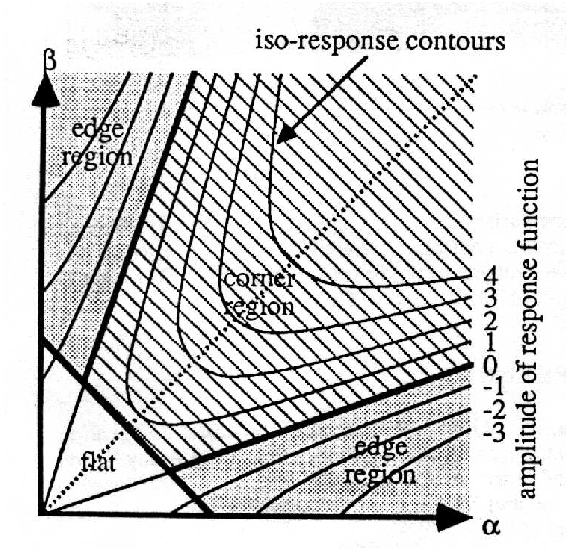
\includegraphics{R}}
		\caption{Nature the point as a function of $\alpha$ and $\beta$.} \label{fig.R}
	\end{figure}

	We can simply define a single scalar value (parametrized by $k$, see below).
	\begin{eqnarray}
		R & = & \det(M)-k.\mbox{tr}^2(M)\\
		  & = & AB-C^2 - k(A+B)^2
	\end{eqnarray}
	Now, corners will be defined as local maxima in the $R$ map.

	\begin{enumerate}
		\item {\bf From previous exercises, compute the maps $A$, $B$ and $C$. }
		\item {\bf Select corner points such that: $k=0.04$ and you simply apply a threshold on the normalized values $R/R_{max}\geq \sigma$ }
		\item {\bf Display the corners as red crosses superimposed on the original image.}
	\end{enumerate}

	{\bf BONUS:}
	\begin{itemize}
		\item What is the influence of the $k$ parameter ?
		\item Add Gaussian and derivative of Gaussian filter instead of $W$ and Sobel filters. Does it enhance the results ?
		\item Do some isotropy comparisons with Moravec: rotate your image a little bit, compute the corners using both approaches and compare.
	\end{itemize}
\end{enumerate}

\end{document}

